% Created 2021-01-21 Thu 06:42
% Intended LaTeX compiler: pdflatex
\documentclass{article}
\usepackage[utf8]{inputenc}
\usepackage[T1]{fontenc}
\usepackage{graphicx}
\usepackage{grffile}
\usepackage{longtable}
\usepackage{wrapfig}
\usepackage{rotating}
\usepackage[normalem]{ulem}
\usepackage{amsmath}
\usepackage{textcomp}
\usepackage{amssymb}
\usepackage{capt-of}
\usepackage{hyperref}
\usepackage[margin=2cm]{geometry}
\usepackage[a4paper,bindingoffset=0.2in,left=1in,right=1in,top=1in,bottom=1in,footskip=.25in]{geometry}
\author{Ricardo Antunes}
\date{January 21, 2021}
\title{Smart Health and Safety Compliance Management for Construction Enterprises - Project Report 01\\\medskip
\large For Internal Use Only}
\hypersetup{
 pdfauthor={Ricardo Antunes},
 pdftitle={Smart Health and Safety Compliance Management for Construction Enterprises - Project Report 01},
 pdfkeywords={},
 pdfsubject={},
 pdfcreator={Emacs 27.1 (Org mode 9.3)}, 
 pdflang={English}}
\begin{document}

\maketitle
\tableofcontents



\section{Proposal summary}
\label{sec:orge4a5b74}

In 2013, The New Zealand Government set a target to reduce work-related fatalities and serious injuries by at least 25\% in seven years. Worksafe, the country's primary workplace health and safety (H\&S) regulator, has used three work-related indicators to measure the progress over this period. The latest official data released by Stats NZ indicated that despite the initial decline two out of these three indicators have bounced back in the past few years (Figure 1), where the construction industry recorded the highest number of incidents related to indicator 2 and the second highest in indicator 3.  

\begin{figure}[htbp]
\centering
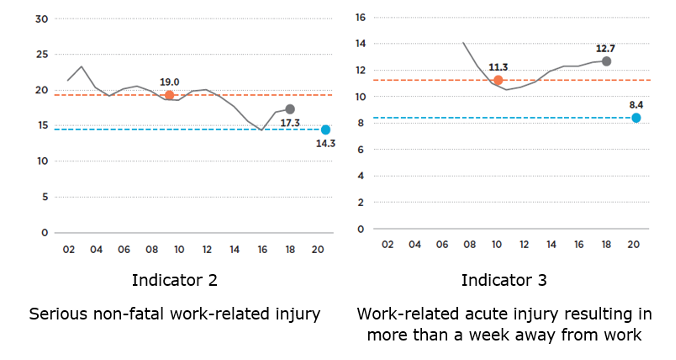
\includegraphics[height=150]{./Images/fig_01.png}
\caption{\label{fig:orgeb6b721}Safety indicators (Source: Stats NZ from ACC claims and Ministry of Health hospitalisation)}
\end{figure}


A review of the current safety management conducts in the construction industry shows them taking stock in individual reporting and filing colossal paperwork.
It makes their output prone to human errors originated either from mistakes or from slips and lapses of memory.
These issues together with the potential physical loss of information present a serious flaw in the system.
Simultaneously, companies are forced to bid with the lowest profit margins to survive in their high competitive environment. Therefore, it is a high priority for every construction company to take up an H\&S compliance management solution that could balance costs, risks and governance.
This proposal aims to complete one step towards sustaining a system that combines the power of machine learning and image processing to "smartify" the risk identification and reporting at the construction sites. Image processing enables the analysis of the safety compliance based on images from the job site.
Machine learning applies artificial intelligence (AI) to automate learning and to improve from experience without being explicitly programmed.
The proposed system provides an accessible and inexpensive solutions operable from the ordinary devices such as the mobile phones with a minimum/ no training period.

\section{Development background}
\label{sec:org01e2406}

This research presents a novel idea in the field of construction H\&S that was initiated by two early-carrier researchers of the Built Environment Engineering department at AUT. It was elaborated further by taking to an external industrial project manager.
The team completed an initial feasibility assessment by testing the capability of the combination of Image processing and machine learning in a particular case (figure 2).
Next, the idea was presented to BRANZ, a major player of research, testing, and consulting in the New Zealand building industry at two steps.
In the first step, a senior scientist of the company investigated the idea, who brought it to the attention of their investment manager.
The second step involved rationalising the definition of a research project based on the proposed idea for the funders. As a result, the team was encouraged to apply for an out of cycle funding subject to providing a proof of concept in the industrial context.
Accordingly, a senior scholar in the computer science department at AUT was invited and joined in mid-2019.
Since then, the team has worked on presenting the idea to the potential stakeholders form the industry. 

\section{Expected outcomes}
\label{sec:orgf3c78d0}

  This study researches into a niche area, leading to contextual benchmarks for smartification of the compliance management in the construction sector.
It can provide useful pointers and information with a contextual transferability of results to the peer domains.

\section{Project delivery}
\label{sec:orgffed39f}
\begin{itemize}
\item Febrary 15th, 2021
\item Required resources (equipment)
\item Schedule of the project delivery: The project period is December 1st, 2020 to February 15th, 2021
\item Estimated total number of hours for delivery of each phase of the project
\item Hourly rate (\$/hrs)
\end{itemize}
\subsection{Duration:}
\label{sec:org87cd193}
\begin{itemize}
\item Weeks: 11
\end{itemize}
\section{Project team}
\label{sec:orgaad9af1}
\begin{enumerate}
\item Dr. Mani Poshdar (mani.poshdar@aut.ac.nz) - Principal Investigator
\item Dr. Ricardo Antunes (ricardo.antunes@aut.ac.nz) - Project Manager / Developer (Application)
\item Dr. Mohammad Norouzifard (mohammad.norouzifard@aut.ac.nz) - Developer (Network)
\end{enumerate}


\section{Project milestones}
\label{sec:orgc3fbdc5}

\begin{center}
\begin{tabular}{llll}
Milestone & Planned date & Status & Actual date\\
\hline
Project kick-off & December 1st, 2020 & Done & January 11th, 2021\\
Data colection &  &  & \\
Data labelling &  &  & \\
System architecture &  &  & \\
Project delivery & February 15th, 2021 &  & \\
 &  &  & \\
\end{tabular}
\end{center}

\section{Project status}
\label{sec:org9fe9779}

\subsection{Scope}
\label{sec:org1042619}

\subsubsection{Data collection}
\label{sec:orgac9c09f}
The data collection has been restricted to data collecteDue to project inactivity and approaching that project delivery date.
The data will now be artificially generated using one webcam, one hard-hat and 1 hight-vizibilty jacket/vest provide by Dr Roohollah Kalatehjari on 20/01/2021.
The recording area in use is WZ level 1.
The approximate installation height of the camera will be 2.20m. 
The recording are will help the developer to prepare the required footages for the training phase. 
\begin{enumerate}
\item Implications on project goal
\label{sec:orged22d82}
The final goal is to provide a prototype that detects if people are using hard-hat and high-visibility jackets/vests at any of the entries of the laboratory area of WZ building.
The accuracy of the system is expected to be inefficient on a construction scenario because of the lack pf approppriate data.
\end{enumerate}


\subsubsection{Resources}
\label{sec:orga344190}
Further to our phone conversations, please arrange to collect the following items from room 801 (WZ level 8) at 12 pm on Wednesday, 20 Jan 2021:

\begin{center}
\begin{tabular}{rl}
Quantitity & Resource\\
\hline
1 & webcam\\
1 & hard hat\\
1 & high-visibility jacket (hi-viz)\\
\end{tabular}
\end{center}

Dr Roohollah Kalatehjari will be there to hand over the items.

As discussed, it will help you to prepare the required footages for the training phase.
We can use WZ level 1 as the recording area. Just to confirm, the final goal is to provide a prototype that detects if people are using hard hat and hi-vis at any of the entries of the laboratory area of WZ building.
The approximate installation height of the camera will be 2.20m.

@Mohammad please confirm your availability to Roo.
@Ricardo Please, keep in touch with Mohammad \& keep the team posted on the progress and any further requirements.
\subsection{Project events}
\label{sec:orgfcbe39c}
\subsubsection{Issue tracker set-up}
\label{sec:org7134b66}
An issue tracking system is a computer software package that manages and maintains lists of issues.
Issue tracking systems are generally used in collaborative settings—especially in large or distributed collaborations—but can also be employed by individuals as part of a time management or personal productivity regime.
\subsubsection{Data collection}
\label{sec:orgda0f92d}
Data is either images or videos where the equipment is show.
The amount, quality and variaty of the data collected impacts had a direct impact on the system accuracy. 
\subsubsection{Data labelling}
\label{sec:orgba9f83a}
The equipment when present on the data has to be labelled.
That means either draw a polygon around each equipment of interest on each image or frame (in the case of video) of the data collection.
\subsubsection{System architecture}
\label{sec:org5c02057}
The system architecture is the conceptual model that defines the structure, behavior, and more views of a system.
An architecture description is a formal description and representation of a system, organized in a way that supports reasoning about the structures and behaviors of the system.
The system architeture depends of the final form of deployment, source format, source resolution, scaliability, among other factors.
\subsubsection{Network design}
\label{sec:org5f01ac8}
The system may contain several networks depending of the funcionalities and system architeture.
\subsubsection{Network training}
\label{sec:orgd1159cf}
Different networks require training methods and efforts.
Training requires preparation and sortout data and prototyping.
\subsubsection{Network evaluation}
\label{sec:orgf4161b1}
Every network should perform with sufficient accuracy.
\subsubsection{Application development}
\label{sec:org562f0da}
Once trained, the network should be wrapped by an application.
That enables the end-user to utilize the system without further requirement other than those instructions presented on the screen.
\subsubsection{Application deployment}
\label{sec:orgfd651b6}
The application deployment involves make the application availabe in a suitable host.
For instance, the application run stand alone on a desktop computer or online as a website or as and mobile phone application.
\subsubsection{Scrum events and project management}
\label{sec:orga91ed48}
Scrum is an agile framework for developing, delivering, and sustaining complex products, with an initial emphasis on software development
It is designed for teams of ten or fewer members, who break their work into goals that can be completed within timeboxed iterations, called sprints, no longer than one month and most commonly two weeks.
At the end of the sprint, the team holds sprint review, to demonstrate the work done, and sprint retrospective to continuously improve.

\subsection{Project schedule}
\label{sec:orgd26a0c8}

\begin{center}
\begin{tabular}{lrrlr}
Description & Planned Effort (h) & Actual Effort (h) & Status & Assigned to\\
\hline
Issue tracker & 0 & 0 & Not started & 3\\
Data collection & 30 & 0 & Not started & 3\\
Data labelling & 50 & 0 & Not started & 3\\
System architecture & 10 & 0 & Not started & 3\\
Network design & 10 & 0 & Not started & 3\\
Network training & 50 & 0 & Not started & 3\\
Network evaluation & 20 & 0 & Not started & 3\\
Network testing & 15 & 0 & Not started & 1,2,3\\
Application development & 0 & 0 & Not started & 2\\
Application deployment & 0 & 0 & Not started & 2\\
Scrum events & 0 & 0 & On going & 1\\
\hline
Total & 185 & 0 & Delayed & \\
\end{tabular}
\end{center}
\end{document}